\documentclass[12pt]{article}
\usepackage{a4wide, amsfonts, epsfig}
\newcommand\soln{\noindent\textit{Solution:} }


%skyline stuff
\font\upright=cmu10 scaled\magstep1
\setlength{\unitlength}{0.012500in}
\begingroup\makeatletter\ifx\SetFigFont\undefined
\def\x#1#2#3#4#5#6#7\relax{\def\x{#1#2#3#4#5#6}}%
\expandafter\x\fmtname xxxxxx\relax \def\y{splain}%
\ifx\x\y   % LaTeX or SliTeX?
\gdef\SetFigFont#1#2#3{%
  \ifnum #1<17\tiny\else \ifnum #1<20\small\else
  \ifnum #1<24\normalsize\else \ifnum #1<29\large\else
  \ifnum #1<34\Large\else \ifnum #1<41\LARGE\else
     \huge\fi\fi\fi\fi\fi\fi
  \csname #3\endcsname}%
\else
\gdef\SetFigFont#1#2#3{\begingroup
  \count@#1\relax \ifnum 25<\count@\count@25\fi
  \def\x{\endgroup\@setsize\SetFigFont{#2pt}}%
  \expandafter\x
    \csname \romannumeral\the\count@ pt\expandafter\endcsname
    \csname @\romannumeral\the\count@ pt\endcsname
  \csname #3\endcsname}%
\fi
\fi\endgroup

\begin{document}
\begin{center}
{\bf 2E2 A sprial example}\footnote{Conor
Houghton, {\tt houghton@maths.tcd.ie} and {\tt
http://www.maths.tcd.ie/\char126 houghton/ 2E2.html}}
\\[1cm]
 5 Febuary 2006
\end{center}
\textsf{
Find the solution of 
\begin{eqnarray}
\frac{dy_1}{dt}&=&y_1-3y_2\\
\frac{dy_2}{dt}&=&3y_1+y_2
\end{eqnarray}
for initial conditions $y_1(0)=r$ and $y_2(0)=0$ write this in real form. Sktech the phase diagram.
\vskip .5cm
\soln This time the matrix is 
$$A=\left(\begin{array}{cc}1&-3\\ 3&1\end{array}\right)$$
and so the spectrum is complex, $\lambda_1=1+3i$ with eigenvector 
$${\bf x}_1=\left(\begin{array}{cc}i\\1\end{array}\right)$$
and $\lambda_2=1-3i$ with eigenvector 
$${\bf x}_2=\left(\begin{array}{cc}-i\\1\end{array}\right)$$
The solution is then
$${\bf y}=\left(\begin{array}{cc}y_1\\y_2\end{array}\right)=c_1\left(\begin{array}{cc}i\\1\end{array}\right)e^{(1+3i)t}+c_2\left(\begin{array}{cc}-i\\1\end{array}\right)e^{(1+3i)t}.$$
Now, this means
$$
\left(\begin{array}{cc}r\\0\end{array}\right)={\bf y}(0)=c_1\left(\begin{array}{cc}i\\1\end{array}\right)+c_2\left(\begin{array}{cc}-i\\1\end{array}\right).$$
and hence $c_1=-ir/2$ and $c_2=ir/2$. Now using $\exp{(a+ib)}=\exp{a}\exp{ib}$ we have solution
$${\bf y}=\frac{r}{2}\left[\left(\begin{array}{cc}1\\-i\end{array}\right)e^{3it}+\left(\begin{array}{cc}1\\i\end{array}\right)e^{-3it}\right]e^{t}.$$
and so
\begin{eqnarray*}
{\bf y}&=&\frac{r}{2}\left[\left(\begin{array}{cc}1\\-i\end{array}\right)(\cos{3t}+i\sin{3t})+\left(\begin{array}{cc}1\\i\end{array}\right)(\cos{3t}-i\sin{3t})\right]e^{t}\\
&=&\left(\begin{array}{cc} r\cos{3t}\\ r\sin{3t}\end{array}\right)e^{t}
\end{eqnarray*}
So, this gives the outwardward spiral. Notice how fast the spiral goes
in. The radius increases exponentially.
\begin{center}
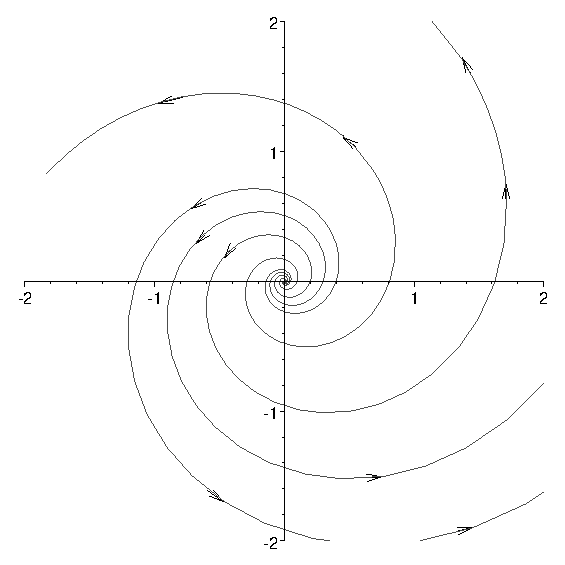
\epsfig{file=27Jan2006.arrowed.eps,width=10cm}
\end{center}
}
\end{document}



